\documentclass[12pt]{exam}
\usepackage[T1]{fontenc}
\usepackage[utf8]{inputenc}
\usepackage{lmodern}
\usepackage[italian]{babel}

\usepackage[margin=1in]{geometry}
\usepackage{amsmath,amssymb}
\usepackage{multicol}

\usepackage{tikz}
\usetikzlibrary{calc}
\def\angolo[#1](#2)(#3:#4:#5)% Syntax: [draw options] (center) (initial angle:final angle:radius)
    { \draw[#1] ($(#2)+({#5*cos(#3)},{#5*sin(#3)})$) arc (#3:#4:#5); }

\newcommand{\class}{Matematica 1 ACC}     %Fisica 5 LS
\newcommand{\examnum}{Verifica 1}               %Verifica 2
\newcommand{\examdate}{15 ottobre 2024}                      %29/10/2018
\newcommand{\timelimit}{1,5 ore}                   %2 ore
\newcommand{\topic}{Numeri naturali e interi}                    %Campo elettrico e campo magnetico

\pagestyle{head}
\firstpageheader{\class}{\examnum\ - Pagina \thepage\ di \numpages}{\examdate}
\runningheader{\class}{\examnum\ - Pagina \thepage\ di \numpages}{\examdate}
\runningheadrule


\begin{document}

\noindent
\begin{tabular*}{\textwidth}{l @{\extracolsep{\fill}} r @{\extracolsep{6pt}} r}
 \textbf{\topic} && \textbf{Durata: \timelimit}\\
 &&\\
 \textbf{Nome:} \makebox[2.9in]{\hrulefill} && \\
\end{tabular*}
\rule[2ex]{\textwidth}{2pt}

% Punteggio totale: \numpoints.
\begin{center}
\addpoints
% \gradetable[v][questions]
\multirowgradetable{1}[questions]
\end{center}

\noindent
\rule[2ex]{\textwidth}{2pt}

\begin{questions}





%DOMANDA SECCA
\question[20] Completa la seguente tabella:
\begin{figure}[h]
    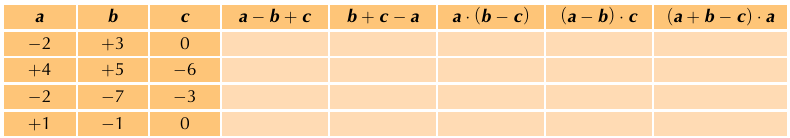
\includegraphics[width=\columnwidth]{img/tabellainteri.png}
  \end{figure}
\addpoints



%DOMANDA DIVISA IN PIÙ RICHIESTE INDICATE CON (a), (b)...
\question[15] Calcola il valore delle seguenti potenze:
\noaddpoints % to omit double points count
\begin{multicols}{3}
\begin{parts}
    \part $ (-3)^2 $
    \part $ (-3)^3 $
    \part $ 5^0 $
\end{parts}
\end{multicols}
\addpoints


%DOMANDA DIVISA IN PIÙ RICHIESTE INDICATE CON (a), (b)...
\question[10] Individua il valore di $ x $ in modo che le seguenti uguaglianze siano vere:
\noaddpoints % to omit double points count
\begin{multicols}{2}
\begin{parts}
    \part $ 3^{9-x} = 81 $
    \part $ 2^{6+x} = 256 $
\end{parts}
\end{multicols}
\addpoints



%DOMANDA DIVISA IN PIÙ RICHIESTE INDICATE CON (a), (b)...
\question[10] Inserisci al posto dei puntini il numero mancante:
\noaddpoints % to omit double points count
\begin{multicols}{2}
\begin{parts}
    \part $ (-9) \cdot (\ldots) = +108 $
    \part $ (+3) \cdot (\ldots) = -48 $
\end{parts}
\end{multicols}
\addpoints


%RISPOSTA MULTIPLA CON BOXES O ALTRO
{%
\checkboxchar{$\Box$} % changing checkbox style locally
\question[15] Quali delle seguenti affermazioni sono vere?
\addpoints
\begin{multicols}{2}
\begin{checkboxes}
    \choice $ 4^4 \cdot 3^4 = 7^4 $
    \choice $ 12^2 : 4^2 = 9 $
    \choice $ 2^5 : 4 = 8 $
    \choice $ (8^3)^2 = 8^5  $
    \choice $ 3^7 \cdot 3^3 : 3^9 = 3 $
    \choice $ 2^{10} \cdot 5^{10} = 10^{10} $
\end{checkboxes}
\end{multicols}
}%



%DOMANDA DIVISA IN PIÙ RICHIESTE INDICATE CON (a), (b)...
\question[30] Calcola il valore delle seguenti espressioni:
\noaddpoints % to omit double points count
\begin{parts}
    \part $ 1 + [(15 : 3) \cdot 7+ (10 \cdot 2): 4] : (2\cdot4) - [(2\cdot5): 2 - 2] $
    
    \hspace{\fill}[$ 3 $]
    \part $ [(3^6 : 3^4) - 2^3] \cdot [(5^3 \cdot 5^4) : (5^2 \cdot 5^3)] : (2^2 + 1) $
    
    \hspace{\fill}[$ 5 $]
    \part $ \{[(-8)^2]^5\}^3 : \{[(-8)^3]^2\}^5 $
    
    \hspace{\fill}[$ 1 $]%203
\end{parts}
\addpoints



\end{questions}

\end{document}
